
% under what circumstances the analysis was carried out?
The needfinding began by analyzing the stakeholders of the research. We started to think from the point of view of an IT office environment, because this is an area where our team members had personal experience and interest. However, we did not limit our analysis and extended to other fields, for example banking, law and libraries. 

	\begin{figure}[ht] 
		\begin{center}
			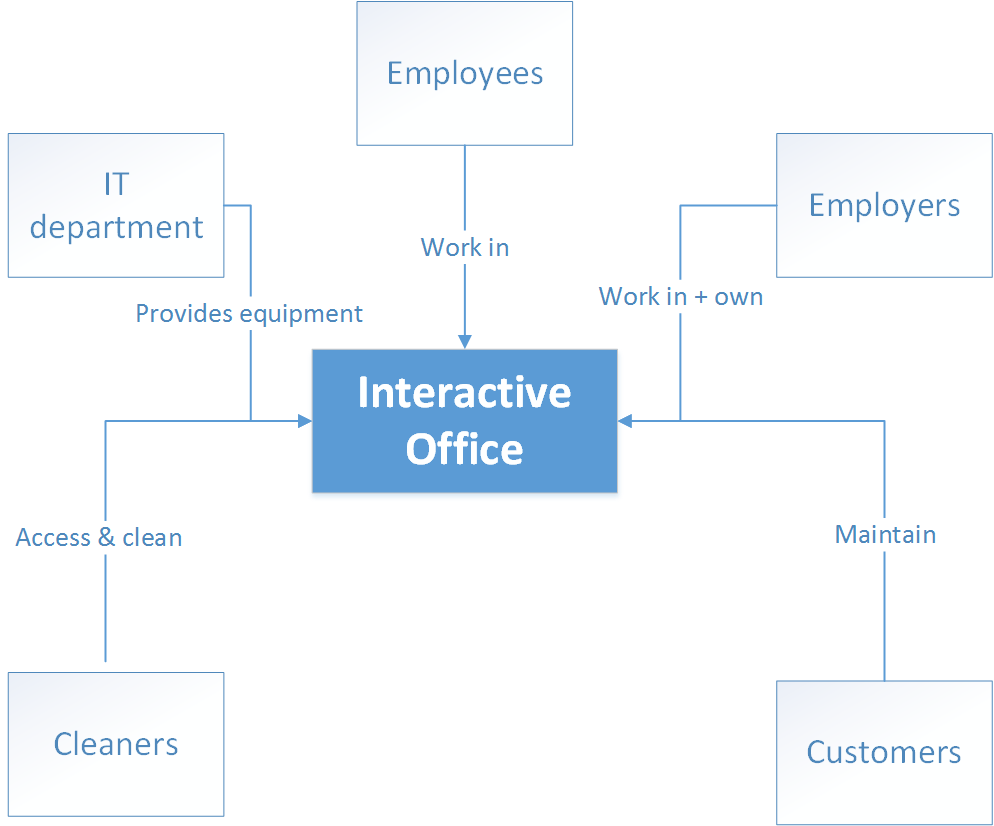
\includegraphics[width=0.9\textwidth]{images/stakeholdermap.png}
			\caption{The stakeholder map in an office environment.}
			\label{stakeholder_map}
		\end{center}
	\end{figure}

% who are the stakeholders? 
During our analysis, the following stakeholders were identified. The stakeholder map is displayed on Figure \ref{stakeholder_map}. 
\begin{enumerate}
	\item Employees
	\item Employers
	\item Customers/Visitors
%Potential and existing customers of the firm
%Business partners, investors
%Third parties, e.g. bank representatives, TEKES, …
%Relatives of employees
%Come to visit the office occasionally
%Stay for a short while
%Meetings, Coffee
%Initial information on the structure of the office
%Where to find the meeting room/person (s)he came to meet
%aula to wait for the person if busy
%(AI receptionist?)
	\item Cleaners
%Somebody who is cleaning the office
%One or more
%Once a day/week, …
%(AI cleaning robots)
%Optimal path to clean the office
%(sensors to check consumables?)
%(buttons in every room (green/red) which employees can press to “order” cleaning service) -> mobile app for employees
%Lights on when cleaning starts -> lights off in the room when the cleaning is complete and tables green/red indicators
%Number of ordered cleaners corresponds to the rooms marked as to be cleaned
%(Indoor Navigation?)

	\item IT Department
%People responsible for the maintenance of the (IT) infrastructure of the office
%Their goal is to ensure the functionality of the electronics in the office (e.g. lights, air conditioning, heating, …)
%Sensors to expensive devices to indicate if they’re wearing or not -> in case an error occurs, IT department should be notified where the device is and what the problem is
%Tablet can help to find the way to the device
%(Indoor Navigation?)
%Expensive/Valuable devices should stay in the office

\end{enumerate}

% what are the connections between the stakeholders? 
The stakeholders are connected through the office environment with slightly different needs. For example, a regular employee in the office experiences different means and performs other kinds of tasks than a cleaning lady. Nevertheless, a common purpose is the efficient and precise completion of work-related activities for all parties. Individuals may interact with one another and have to perform tasks collaboratively, together. The infrastructure that is provided by the office may be shared and used by multiple parties. 

Therefore, we concluded that the collaboration, interaction and the proper facilities in the office are essential aspects to carry on with the research. On top of that, the environment has to facilitate efficient work as well as quality outcome of all parties. As a future vision, we imagined an interactive office environment that facilitates all the aspects and needs covered by the stakeholders above. 

% what was excluded?
On top of the stakeholders listed above and displayed on Figure \ref{stakeholder_map}, other parties were identified. For instance, we were thinking of how the Worker's Union or security companies may benefit from a more interactive office environment, however we concluded that such analysis is out of the scope of our research. Therefore, our focus was moved towards other directions. 